\documentclass{article}
\usepackage[utf8]{inputenc}
\usepackage[T1]{fontenc} % Use 8-bit encoding that has 256 glyphs
\usepackage{fourier} % Use the Adobe Utopia font for the document - comment this line to return to the LaTeX default
\usepackage[english]{babel} % English language/hyphenation
\usepackage{amsmath,amsfonts,amsthm} % Math packages
\usepackage{changepage}
\usepackage{graphicx}
\usepackage{sectsty} % Allows customizing section commands
\usepackage{qtree}
\allsectionsfont{\centering \normalfont\scshape} % Make all sections centered, the default font and small caps
\usepackage{algorithm2e}
\usepackage{fancyhdr} % Custom headers and footers
\pagestyle{fancyplain} % Makes all pages in the document conform to the custom headers and footers
\fancyhead{} % No page header - if you want one, create it in the same way as the footers below
\fancyfoot[L]{} % Empty left footer
\fancyfoot[C]{} % Empty center footer
\fancyfoot[R]{\thepage} % Page numbering for right footer
\renewcommand{\headrulewidth}{0pt} % Remove header underlines
\renewcommand{\footrulewidth}{0pt} % Remove footer underlines
\setlength{\headheight}{13.6pt} % Customize the height of the header

\numberwithin{equation}{section} % Number equations within sections (i.e. 1.1, 1.2, 2.1, 2.2 instead of 1, 2, 3, 4)
\numberwithin{figure}{section} % Number figures within sections (i.e. 1.1, 1.2, 2.1, 2.2 instead of 1, 2, 3, 4)
\numberwithin{table}{section} % Number tables within sections (i.e. 1.1, 1.2, 2.1, 2.2 instead of 1, 2, 3, 4)

\setlength\parindent{0pt} % Removes all indentation from paragraphs - comment this line for an assignment with lots of text

%----------------------------------------------------------------------------------------
% TITLE SECTION
%----------------------------------------------------------------------------------------

\newcommand{\horrule}[1]{\rule{\linewidth}{#1}} % Create horizontal rule command with 1 argument of height

\title{
\large{\textsc{University of Victoria Computer Science}}\huge\\ [0pt] % Your university, school and/or department name(s)
\horrule{0.5pt}\\[0.4cm]
\textsc{Csc586A Theoretical Models\\Final Exam}\\
\author{Braden Simpson\\braden@uvic.ca\\V00685500}
\date{August 6, 2013}
}

\begin{document}

\maketitle % Print the title

\section{Question One}
\label{sec:one}
\subsection{Part A}
In this course, the theoretical model I chose to study most was for the project that Jordan and I did, and that model is the Abstract Syntax Tree (AST), more specifically, algorithms to find edit distances between them.  The AST is a tree represents the syntactic structure of source code, where each node is a construct (while, return, if etc.), leaves are variables, and branches are blocks of code.  See Appendix ~\ref{app:one} for an example.

By using these trees and the algorithms for edit distance, outlined by the fluri et al. \cite{fluri}, we were able to implement an algorithm for finding the changes between two ASTs.  I learned from the literature how to perform algorithms on these ASTs to find matching leaves, using levehnstein, n-grams, and other measures.

I also studied procedural generation and markov chains, but they weren't as in depth as the the trees.  I found the procedural generation algorithms such as L-Systems and Noise generation to be particularly interesting, especially because of their real-world use in video games and simulations.  Because the framework for L-Systems is so easy to learn, anybody can envision how they might be used in nature, which is sometimes hard to do when talking about theoretical models.

\subsection{Part B}
I used multiple different sources for my work, most of all the paper which helped us learn the algorithms required to perform tree edit distance calculations from fluri et al. \cite{fluri}.  As well I used different research on MSR conferences to learn how to analyze and interpret the data correctly, even as I was there this year, seeing the different ways people inetepret datasets has given me the insight required to critically assess what the data means, what inferences we can get, and more importantly, what we cannot get.  

\subsection{Part C}
\label{sec:q1c}
For this section I will do an example run of our algorithm for finding the change types in two ASTs for a file (before and after).  This will show how the algorithms are used to 


\begin{center}
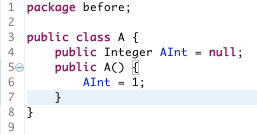
\includegraphics[width=0.5\linewidth]{codebefore}
\label{fig:cbefore}\\
The code for class A before a change.

\scriptsize
\Tree[.NAME(before.A) [.BODY\_DECLARATIONS  [.FieldDeclaration    [.Fragments \textit{A.Aint} ]
                                                                  [.Type \textit{java.lang.Integer} ]
                                                                  [.Modifiers \textit{public} ]]
                                            [.MethodDeclaration   [.Modifiers \textit{public} ]
                                                                  [.Name \textit{A.A()} ]
                                                                  [.Body [.Statement [.Expression [.LHS \textit{A.AInt} ]
                                                                                                  [.Operator \textit{'='} ]
                                                                                                  [.RHS [.ConstantValue \textit{1} ]]]]]]]]
\normalsize
\\
The AST that corresponds to Figure ~\ref{fig:cbefore}
\end{center}

\begin{center}
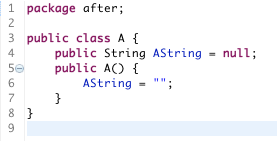
\includegraphics[width=0.5\linewidth]{codeafter}
\label{fig:cafter}\\
The code for class A after a change.

\scriptsize
\Tree[.NAME(after.A) [.BODY\_DECLARATIONS   [.FieldDeclaration    [.Fragments \textit{A.AString} ]
                                                                  [.Type \textit{java.lang.String} ]
                                                                  [.Modifiers \textit{public} ]]
                                            [.MethodDeclaration   [.Modifiers \textit{public} ]
                                                                  [.Name \textit{A.A()} ]
                                                                  [.Body [.Statement [.Expression [.LHS \textit{A.AString} ]
                                                                                                  [.Operator \textit{'='} ]
                                                                                                  [.RHS [.ConstantValue \textit{""} ]]]]]]]]
\normalsize
\\
The AST that corresponds to Figure ~\ref{fig:cafter}
\end{center}


Once we have the two ASTs, we use methods in \cite{fluri} to match the nodes, using Levehnstein and n-gram similarity, to match the nodes.  Then we apply our rules, to find an edit script, namely what we need to do to get $Tree_1$ to $Tree_2$.  


\footnotetext{Note that for Section~\ref{sec:q1c} I omitted a few nodes in the ASTs for simplicity, there are many that are generated by the JVM.}



\section{Question Two}

\appendix
\section{Abstract Syntax Trees}
\label{app:one}
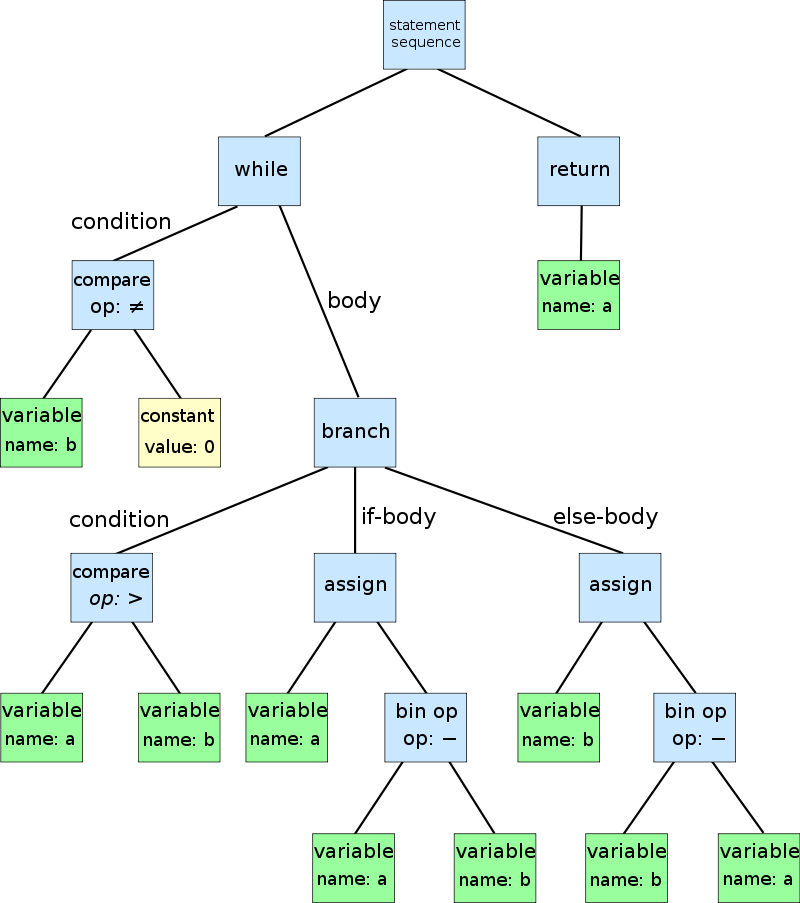
\includegraphics[width=\textwidth]{diff.png}\\

\begin{algorithm}[H]
 \SetAlgoLined
 \KwData{An abstract syntax tree with matching psuedocode for Euclidean Algorithm.  Taken from the wikipedia entry ~\cite{wiki}}
 \While{b $\neq$ 0}{
  \eIf{a > b}{
    a = a - b      
  }{
    b = b - a
  }
}
return a
\end{algorithm}
\bibliographystyle{IEEEtran}
\bibliography{final} 
\end{document}